\def\objectdetection{
    \section{Các mô hình giải quyết bài toán object detection}
    Các mô hình giải quyết bài toán object detection theo kiến trúc mô hình thường được chia thành hai nhóm: nhóm các mô hình two-stage và nhóm các mô hình single-stage.

    \noindent
    Các mô hình two-stage giải quyết bài toán object detection có đặc điểm chung về kiến trúc mô hình gồm hai phần: \\
    - Phần thứ nhất được gọi là \textit{Region proposals module}, mô đun nhận đầu vào là ảnh ban đầu và trả đầu ra giúp đề xuất ra các khu vực trên ảnh mà có khả năng chứa đối tượng. \\
    - Phần thứ hai được gọi là \textit{Feature extraction module}, mô đun nhận đầu vào là kết quả của Region proposals module giúp xác định chính xác đối tượng trong khu vực đó là đối tượng nào và tinh chỉnh toạ độ của khu vực chính xác hơn. \\

    Nổi bật trong nhóm các mô hình two-stage là nhóm các mô hình R-CNN, Fast R-CNN và Faster R-CNN.

    \subsection{Nhóm các mô hình R-CNN, Fast R-CNN và Faster R-CNN}

    \def\rcnn{
    \subsubsection{Mô hình R-CNN}
    Một trong các mô hình đầu tiên ứng dụng học sâu giải quyết bài toán object detection là Regions with CNN features \cite{girshick2014rich} (gọi tắt là R-CNN).
    Tuy nhiên, ở thời điểm mà mô hình R-CNN ra đời, do các mô hình học sâu chưa thật sự phát triển nên mô hình R-CNN không hoàn toàn sử dụng học sâu mà vẫn dựa trên kết quả của thuật toán xử lý ảnh như Graph-Based Image Segmentation \cite{felzenszwalb2004efficient} và Selective Search \cite{uijlings2013selective}.

    \noindent
    \textbf{\textit{Thuật toán Graph-Based Image Segmentation}} \\

    \noindent
    \textbf{\textit{Thuật toán Selective Search}} \\
    
    \noindent
    \textbf{\textit{Kiến trúc mô hình R-CNN}} \\
    Là một trong số các mô hình two-stage, mô hình R-CNN bao gồm hai thành phần: \\
    - Phần Region proposals module mà mô hình R-CNN sử dụng là thuật toán Selective Search ở trên.
    Nhận đầu vào là ảnh, thuật toán Selective Search trả đầu ra là khoảng 2000 khu vực có khả năng có chứa đối tượng và mô hình R-CNN sử dụng các khu vực này làm đầu vào cho thành phần thứ hai. \\
    - Phần Feature extraction module của mô hình R-CNN là một mô hình phân lớp ảnh, cụ thể theo \cite{girshick2014rich} là AlexNet.
    Mô hình R-CNN sử dụng AlexNet nhằm đánh giá xem khu vực đã được đề xuất bởi Selective Search có chứa đối tượng hay không và nếu có thì khu vực đó chứa đối tượng nào. \\

    \begin{figure}[H]
        \centering
        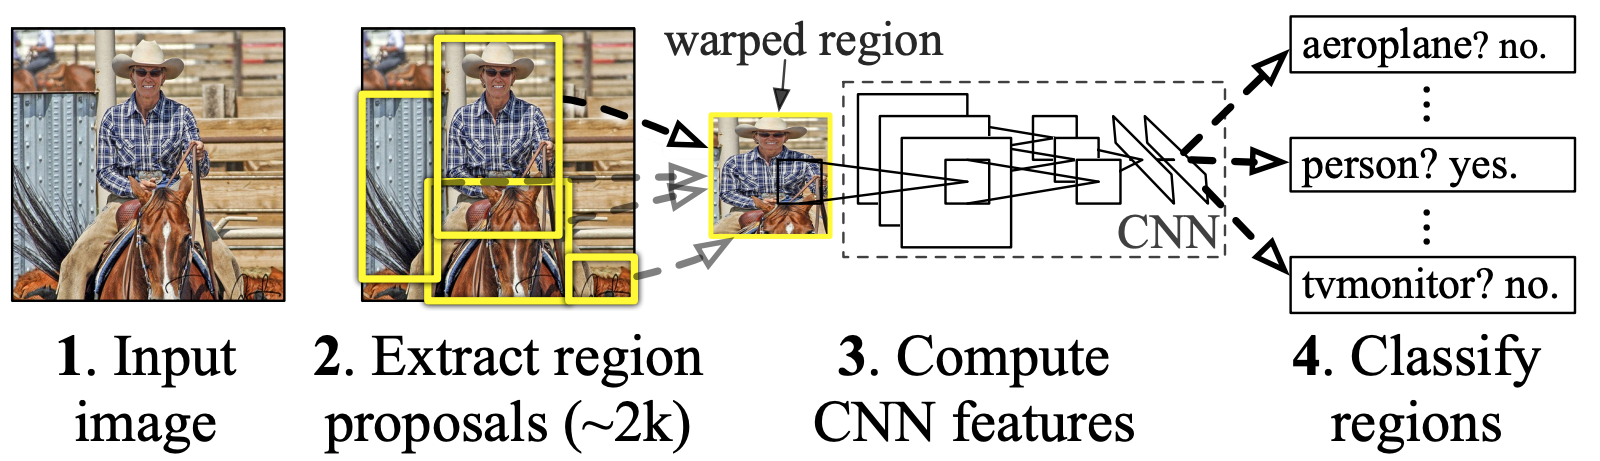
\includegraphics[width=13cm] {images/rcnn_model}
        \caption{Kiến trúc mô hình R-CNN (Nguồn: \cite{girshick2014rich})}
        \label{fig:rcnn_model}
    \end{figure}

    \noindent
    Đối với thành phần Feature extraction module, nhóm tác giả thực hiện hai thí nghiệm: \\
    \textit{Thí nghiệm 1: Finetune mô hình phân lớp CNN} \\
    Nhóm tác giả thay thế lớp fully-connected cuối cùng của mô hình AlexNet (gồm 1000 lớp theo bộ dữ liệu ImageNet) bằng một lớp fully-connected mới (gồm 21 lớp: 20 lớp của bộ dữ liệu VOC và 1 lớp ứng với background).
    Và họ finetune lại mô hình này với thuật toán tối ưu là SGC và learning rate rất nhỏ.
    Các khu vực đã được đề xuất bởi thuật toán Selective Search được sử dụng làm dữ liệu cho bước này, trong đó:
    Những khu vực có chỉ số IoU với groundtruth bounding box >= 0.5 được gán nhãn là lớp của bounding box đó.
    Và ngược lại, sẽ được gán nhãn là lớp background. \\
    TODO Appendix B \\
    Lý do ta cần finetune lại mô hình AlexNet được nhóm tác giả giải thích rằng có những điểm khác nhau giữa bộ dữ liệu pretrained ImageNet và bộ dữ liệu gồm các khu vực được đề xuất bởi Selective Search.

    \noindent
    \textit{Thí nghiệm 2: Xây dựng bộ phân lớp đối tượng bằng SVM} \\
    Với mô hình AlexNet đã được finetune lại như trên, nhóm tác giả sử dụng nó để lấy ra các đặc trưng của ảnh đầu vào và từ đó train các mô hình SVM.
    Mỗi mô hình SVM tương ứng với một lớp đối tượng và mỗi mô hình SVM trả lời cho câu hỏi, đặc trưng của khu vực đó có phải là đối tượng đó hay không.
    Những đặc trưng của khu vực có chỉ số IoU với groundtruth bounding box >= 0.3 sẽ được gán nhãn là lớp của bounding box đó.
    Và ngược lại, những đặc trưng của khu vực có chỉ số IoU với groundtruth bounding box < 0.3 sẽ được gán nhãn không phải là lớp của bounding box đó. \\
    TODO Appendix B \\

    \textit{Bước 3 (Tuỳ chọn)}: Bổ sung thêm hàm loss cải thiện khả năng định vị khu vực \\
    TODO Appendix C \\

    \noindent
    \textbf{\textit{Kết quả của mô hình R-CNN}} \\
    Kết quả của mô hình R-CNN trên bộ dữ liệu VOC 2010 test rất đáng chú ý.
    Trong hình \ref{fig:rcnn_results_3}, ta xét đến hai cấu hình của mô hình R-CNN: \\
    - Cấu hình cơ bản không bao gồm bước Bổ sung thêm hàm loss cải thiện khả năng định vị khu vực được gọi là R-CNN. \\
    - Cấu hình nâng cao Bổ sung thêm hàm loss cải thiện khả năng định vị khu vực được gọi là R-CNN BB. \\
    Với cấu hình cơ bản, R-CNN đạt được chỉ số average precision cao hơn trên tất cả các lớp đối tượng và chỉ số mAP cao hơn 10\% so với các mô hình hiện đại nhất tại thời điểm đó.
    Hơn nữa, với cấu hình R-CNN BB, mô hình còn đạt được chỉ số AP trên tất cả các lớp đối tượng và chỉ số mAP cao hơn 3\% so với cấu hình cơ bản R-CNN.
    \begin{figure}[H]
        \centering
        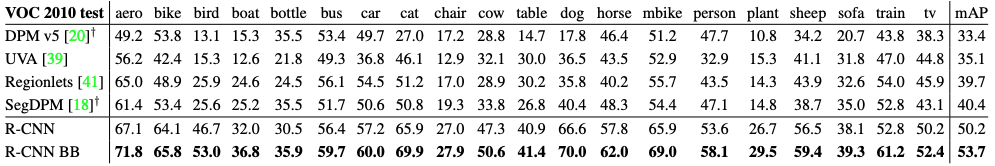
\includegraphics[width=15cm] {images/rcnn_results_3}
        \caption{Kết quả của mô hình R-CNN trên bộ dữ liệu VOC 2010 test. So sánh kết quả của R-CNN và của các mô hình khác nhau (Nguồn: \cite{girshick2014rich})}
        \label{fig:rcnn_results_3}
    \end{figure}
    \noindent
    Ngoài ra, nhóm tác giả cũng nghiên cứu kết quả giữa các cấu hình khác nhau của mô hình R-CNN.
    Trong hình \ref{fig:rcnn_results_1}, nhóm tác giả xét đến hai nhóm cấu hình khác nhau: \\
    - Nhóm cấu hình không finetune và sử dụng đặc trưng ở các vị trí khác nhau cho mô hình phân lớp SVM: \par
    + Cấu hình lấy đặc trưng ở lớp pooling thứ 5: R-CNN ${pool}_{5}$. \par
    + Cấu hình lấy đặc trưng ở lớp fully-connected thứ 6: R-CNN ${fc}_{6}$. \par
    + Cấu hình lấy đặc trưng ở lớp fully-connected thứ 7: R-CNN ${fc}_{7}$. \\
    - Nhóm cấu hình có finetune và sử dụng đặc trưng ở các vị trí khác nhau cho mô hình phân lớp SVM: \par
    + Cấu hình lấy đặc trưng ở lớp pooling thứ 5: R-CNN FT ${pool}_{5}$. \par
    + Cấu hình lấy đặc trưng ở lớp fully-connected thứ 6: R-CNN FT ${fc}_{6}$. \par
    + Cấu hình lấy đặc trưng ở lớp fully-connected thứ 7: R-CNN FT ${fc}_{7}$. \par
    + Cấu hình lấy đặc trưng ở lớp fully-connected thứ 7 kết hợp với hàm loss cải thiện khả năng định vị khu vực: R-CNN FT ${fc}_{7}$ BB. \\
    Với việc finetune lại mô hình với dữ liệu VOC, nhóm cấu hình có finetune mang lại kết quả tốt hơn rất nhiều.
    Trong việc lựa chọn vị trí lấy đặc trưng, vị trí lớp fully-connected thứ 6 là tốt nhất trong nhóm các mô hình không finetune.
    Còn đối với nhóm các mô hình có finetune, vị trí lớp fully-connected thứ 7 là mô hình có kết quả tốt nhất.
    Kết hợp tất cả các kết quả trên, cấu hình R-CNN FT ${fc}_{7}$ BB cho kết quả tốt nhất so sánh với tất cả các cấu hình khác.
    \begin{figure}[H]
        \centering
        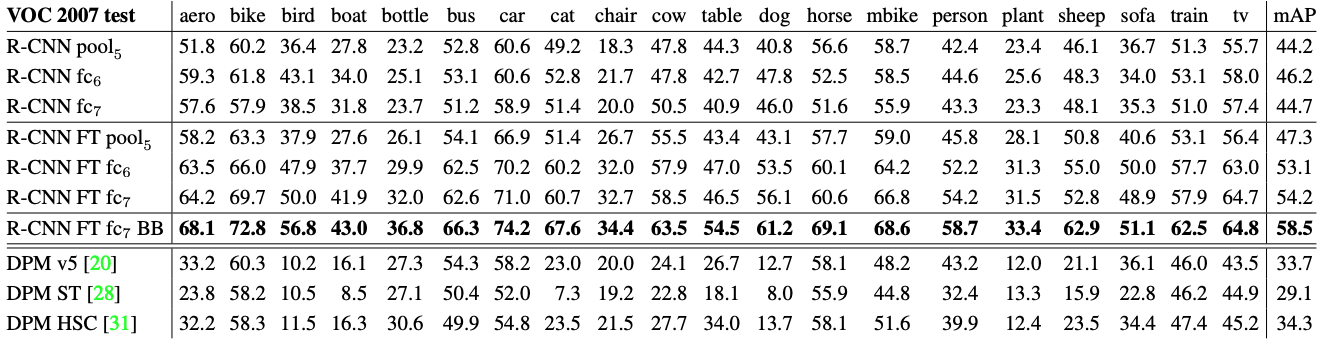
\includegraphics[width=15cm] {images/rcnn_results_1}
        \caption{Kết quả của mô hình R-CNN trên bộ dữ liệu VOC 2007 test. So sánh kết quả của các cấu hình khác nhau của mô hình R-CNN và của mô hình DPM (Nguồn: \cite{girshick2014rich})}
        \label{fig:rcnn_results_1}
    \end{figure}
    \noindent
    Cuối cùng, nhóm tác giả so sánh vai trò của Feature extraction module đối với kết quả chung của mô hình R-CNN.
    Trong hình \ref{fig:rcnn_results_2}, nhóm tác giả xét đến hai mô hình có thể sử dụng trong Feature extraction module: \\
    - Cấu hình sử dụng mô hình AlexNet: R-CNN T-Net và R-CNN T-Net BB. \\
    - Cấu hình sử dụng mô hình VGG16: R-CNN O-Net và R-CNN O-Net BB. \\
    Trong thí nghiệm này, mô hình VGG16 cho kết quả tốt hơn khá nhiều so với mô hình AlexNet.
    \begin{figure}[H]
        \centering
        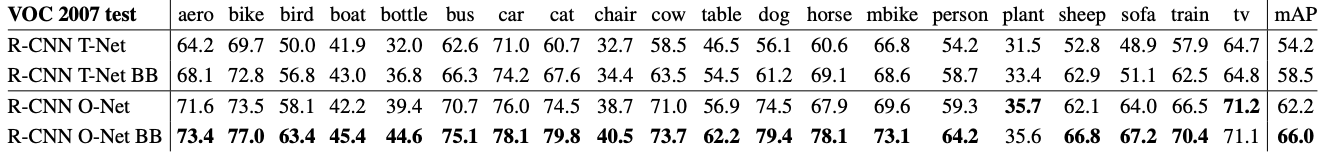
\includegraphics[width=15cm] {images/rcnn_results_2}
        \caption{Kết quả của mô hình R-CNN trên bộ dữ liệu VOC 2007 test (Nguồn: \cite{girshick2014rich})}
        \label{fig:rcnn_results_2}
    \end{figure}

    \noindent
    \textbf{\textit{Vấn đề tồn đọng của mô hình R-CNN}} \\
    Vấn đề lớn nhất của mô hình R-CNN là thời gian mà mô hình cần cho quá trình train và quá trình test là rất lớn.
    Trong quá trình test, mô hình R-CNN sử dụng tới 47 giây để hoàn thành việc xử lý một ảnh.
    Kết quả này khiến cho mô hình R-CNN gần như không có giá trị thực tiễn.
}
    \rcnn

    \def\fastrcnn{
    Fast R-CNN \cite{girshick2015fast}, được phát triển bởi một trong nhóm tác giả của mô hình R-CNN, và là một phiên bản nâng cấp hơn so với R-CNN giúp phần nào giải quyết được một phần điểm yếu về tốc độ của mô hình R-CNN.

    \subsubsection*{Kiến trúc mô hình Fast R-CNN}
    Là một phiên bản nâng cấp của mô hình R-CNN, nên Fast R-CNN cũng bao gồm hai thành phần: \\
    - Phần region proposals module \index{region proposals module} mà mô hình Fast R-CNN sử dụng vẫn là thuật toán Selective Search tương tự như R-CNN. \\
    - Phần feature extraction module \index{feature extraction module} của mô hình R-CNN là một mô hình phân lớp ảnh, cụ thể theo \cite{girshick2015fast} là VGG16. \\
    Các thành phần của mô hình Fast R-CNN không có thay đổi gì quá nổi bật so với R-CNN, tuy nhiên, điểm khác biệt mang lại giá trị của Fast R-CNN nằm ở cách mà mô hình này kết hợp hai thành phần trên.

    \begin{figure}[H]
        \centering
        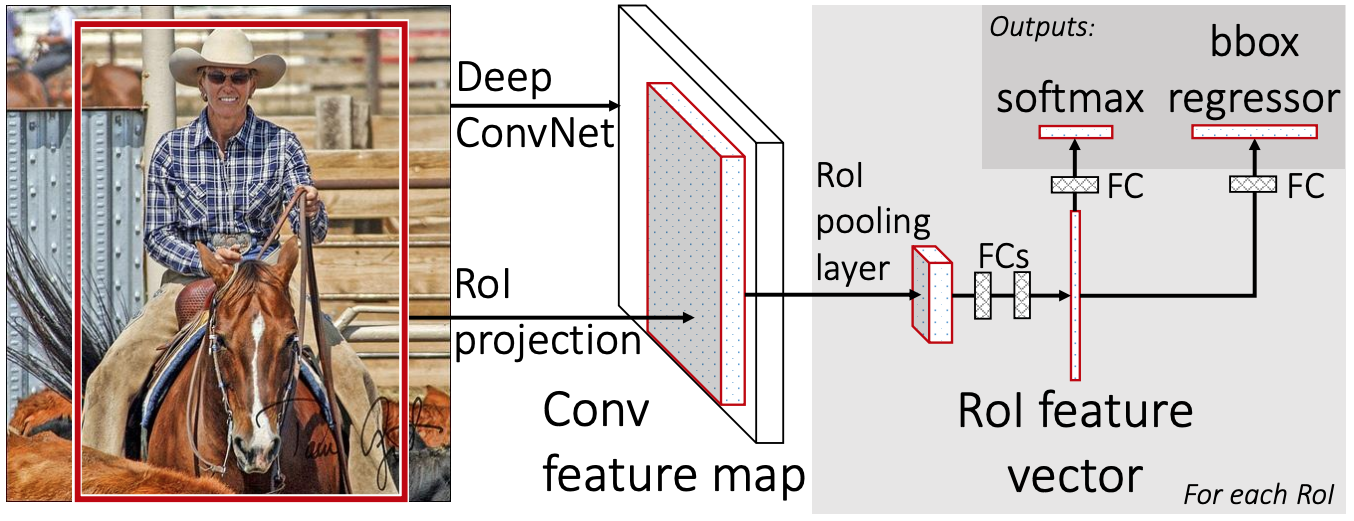
\includegraphics[width=13cm] {images/fast_rcnn_model}
        \caption{Kiến trúc mô hình Fast R-CNN (Nguồn: \cite{girshick2015fast})}
        \label{fig:fast_rcnn_model}
    \end{figure}

    \noindent
    Khác với R-CNN, mô hình Fast R-CNN đưa toàn bộ ảnh ban đầu qua các lớp conv và pooling của feature extraction module \index{feature extraction module} để tạo ra được đặc trưng của toàn bộ ảnh.
    Tiếp theo, với mỗi khu vực mà thuật toán Selective Search đề xuất (các khu vực này, theo \cite{girshick2015fast}, gọi là các \textit{regions of interest} hay \textit{RoIs}), mô hình Fast R-CNN trích xuất từ đặc trưng của toàn bộ ảnh ra đặc trưng đại diện cho khu vực đề xuất đó.
    Cuối cùng, mỗi đặc trưng đại diện cho mỗi khu vực đề xuất được đưa qua các lớp fully-connected và trả hai đầu ra gồm giá trị xác suất khu vực đó là đối tượng nào và giá trị độ lệch của bounding box \index{bounding box}. \\
    Tuy nhiên, có một vấn xảy ra với cách thiết kế mô hình trên, đó là mỗi khu vực đề xuất từ thuật toán Selective Search có kích thước khác nhau, do đó, kích thước của đặc trưng đại diện cho mỗi khu vực đề xuất cũng khác nhau và ta cần các đặc trưng này có cùng kích thước để có thể đưa vào cùng chung các lớp fully-connected.
    Tác giả giải quyết vấn đề này bằng cách xây dựng một lớp mới trong kiến trúc mô hình Fast R-CNN, tên là \textit{RoI pooling}.

    \subsubsection*{Lớp RoI pooling}
    Trước khi đi sâu vào chi tiết của lớp RoI pooling, ta sẽ cùng bàn luận về lớp pooling thông thường.
    Có hai phương pháp pooling phổ biến là max pooling và average pooling.

    \begin{figure}[H]
        \centering
        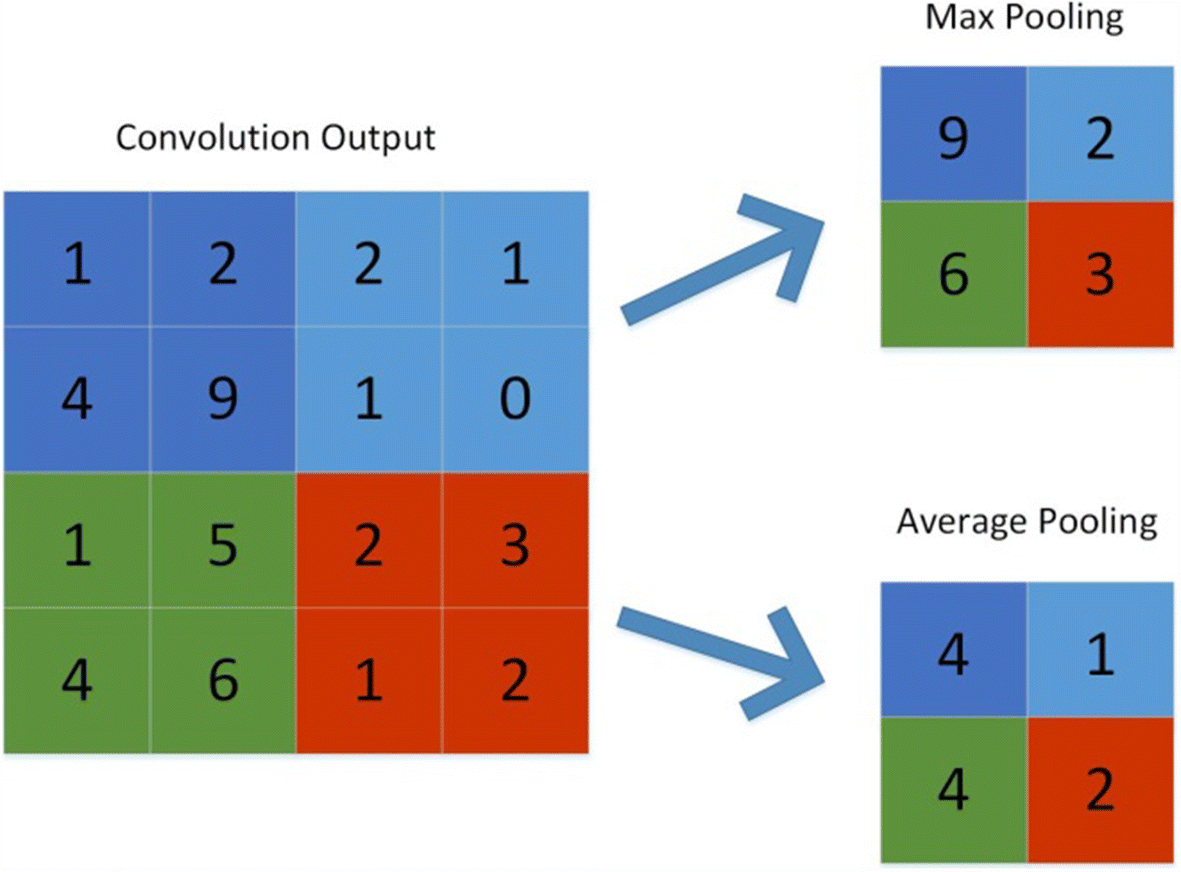
\includegraphics[width=8cm] {images/pooling}
        \caption{Kết quả sau khi thực hiện max pooling và average pooling (Nguồn: media.springernature.com)}
        \label{fig:pooling}
    \end{figure}

    \noindent
    Tuy nhiên, hai phương pháp trên đều có cách thực hiện dựa trên kernel và stride, nghĩa là kích thước của đặc trưng sau khi đi qua lớp pooling phụ thuộc vào kích thước đặc trưng trước khi đi qua lớp pooling, kích thước của kernel pooling và kích thước của stride pooling. \\
    Cụ thể hơn, với một đặc trưng từ lớp conv có kích thước chiều rộng và chiều cao lần lượt là ${W}_{1}$ và ${H}_{1}$ và lớp pooling có kích thước kernel là K, kích thước stride là S, ta sẽ thu được đặc trưng sau khi đi qua lớp pooling này có kích thước chiều rộng và chiều cao lần lượt là ${W}_{2} = \frac{{W}_{1} - (K - 1) - 1}{S} + 1$ và ${H}_{2} = \frac{{H}_{1} - (K - 1) - 1}{S} + 1$.

    \begin{figure}[H]
        \centering
        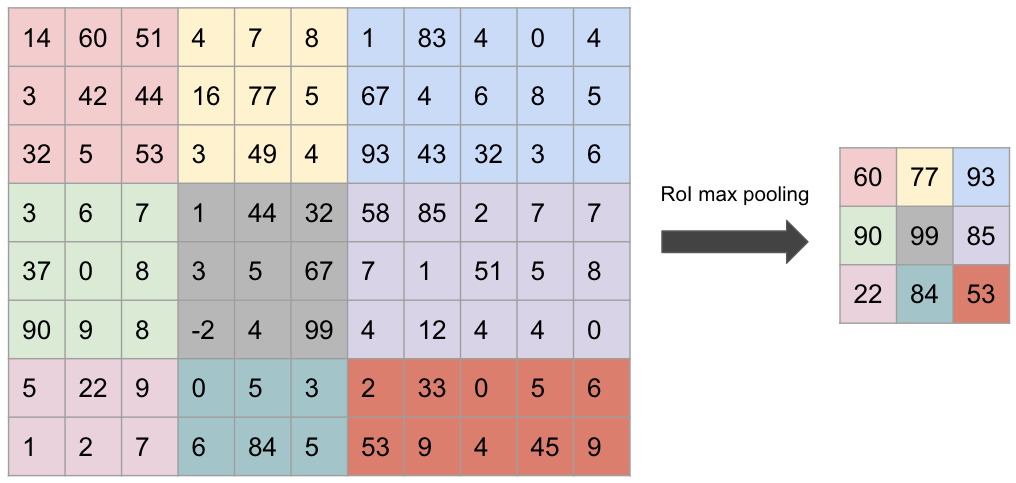
\includegraphics[width=10cm] {images/roi_pooling}
        \caption{Kết quả sau khi thực hiện RoI max pooling}
        \label{fig:roi_pooling}
    \end{figure}

    \noindent
    Trong khi đó, RoIs pooling được giới thiệu bởi tác giả không hoạt động như vậy.
    Thay vì yêu cầu ta phải định nghĩa kích thước kernel và kích thước stride, RoI pooling yêu cầu ta phải định nghĩa kích thước của đặc trưng đầu ra, từ đó, RoI pooling sẽ tính toán và chia đặc trưng đầu vào thành các vùng trước khi thực hiện phép max pooling. \\
    Cụ thể hơn, với một đặc trưng từ lớp conv có kích thước chiều rộng và chiều cao lần lượt là ${W}_{1}$ và ${H}_{1}$ và ta định nghĩa kích thước của đặc trưng đầu ra có kích thước chiều rộng và chiều cao lần lượt là ${W}_{2}$ và ${H}_{2}$, RoI pooling sẽ tính toán được kích thước và vị trí của từng khu vực pooling: \\
    - Theo chiều W, ta có ${W}_{2}$ phần pooling và mỗi phần có kích thước là ${K}_{w} = \lfloor\frac{{W}_{1}}{{W}_{2}}\rfloor$, ngoại trừ phần cuối có kích thước ${K}_{w} + ({W}_{1} - {W}_{2} * {K}_{w})$. \\
    - Theo chiều H, ta có ${H}_{2}$ phần pooling và mỗi phần có kích thước là ${K}_{h} = \lfloor\frac{{H}_{1}}{{H}_{2}}\rfloor$, ngoại trừ phần cuối có kích thước ${K}_{h} + ({H}_{1} - {H}_{2} * {K}_{h})$. \\

    \subsubsection*{Hàm loss multi-task và cách finetune mô hình Fast R-CNN}
    Một điểm cải tiến khác của mô hình Fast R-CNN so với mô hình R-CNN đó là việc sử dụng hàm loss multi-task và finetune toàn bộ mô hình. \\
    Trong quá trình huấn luyện mô hình, tác giả lấy ngẫu nhiên N ảnh và lấy ngẫu nhiên $\frac{R}{N}$ RoIs trên mỗi ảnh.
    Nhằm đảm bảo vấn đề về bộ nhớ không xảy ra trong suốt quá trình huấn luyện, tác giả lựa chọn N = 2 và R = 128.
    Ngoài ra, tác giả cũng đề cập đến một lo ngại khác, đó là việc sử dụng nhiều RoIs trên một số ít ảnh có thể dẫn đến quá trình tối ưu chậm và mất nhiều thời gian để mô hình đạt được điểm hội tụ.
    Tuy nhiên, trong thực tế, điều này đã không xảy ra. \\
    Mô hình Fast R-CNN có hai lớp đầu ra: \\
    - Một là giá trị xác suất một khu vực nào đó là đối tượng nào $p = (p_0, \dots, p_K)$, tương ứng với $K + 1$ lớp đối tượng \index{lớp đối tượng} ($K$ lớp đối tượng \index{lớp đối tượng} từ bộ dữ liệu và 1 lớp background \index{background}). \\
    - Còn lại là giá trị độ lệch bounding box \index{bounding box} của khu vực đó $t^{k} = (t^{k}_{x}, t^{k}_{y}, t^{k}_{w}, t^{k}_{h})$, tương ứng với $K$ lớp đối tượng \index{lớp đối tượng} từ bộ dữ liệu. \\
    Với groundtruth \index{groundtruth} lớp đối tượng \index{lớp đối tượng} $u$ và groundtruth \index{groundtruth} toạ độ bounding box \index{bounding box} $v$, ta có hàm loss multi-task với mỗi RoI như sau:

    \begin{equation}
        \label{eq:fast_rcnn_loss}
        L(p, u, t^u, v) = L_{cls}(p, u) + \lambda [u \ge 1] L_{loc}(t^u, v)
    \end{equation}

    \noindent
    Hàm loss trên gồm các thành phần: \\
    -  $L_{cls}(p, u) = -\log p_u$ là hàm log loss với groundtruth \index{groundtruth} lớp đối tượng \index{lớp đối tượng} $u$ \\
    -  $[u \ge 1]$ là hàm chỉ định. Thành phần này bằng 1 nếu $u \ge 1$ và bằng 0 trong các trường hợp còn lại. Thành phần này tồn tại nhằm loại bỏ phần hàm loss tính toán độ lệch bounding box \index{bounding box} nếu lớp đối tượng \index{lớp đối tượng} $u = 0$ bởi vì khi đó, $u$ đại diện cho lớp background \index{background}. \\
    -  $L_{loc}(t^u, v)$ là hàm loss tính toán độ lệch giữa groundtruth \index{groundtruth} toạ độ bounding box \index{bounding box} $v = (v_{x}, v_{y}, v_{w}, v_{h})$ và bounding box \index{bounding box} dự đoán $t^u = (t^u_{x}, t^u_{y}, t^u_{w}, t^u_{h})$ tương ứng với groundtruth \index{groundtruth} lớp đối tượng \index{lớp đối tượng} $u$. Mỗi bounding box \index{bounding box} được biểu diễn bởi bốn giá trị, x - toạ độ x của góc trái trên, y - toạ độ y của góc trái trên, w - chiều rộng của bounding box \index{bounding box} và h - chiều cao của bounding box \index{bounding box}.
    Công thức cụ thể của thành phần $L_{loc}(t^u, v)$ như sau:

    \begin{equation}
        \label{eq:fast_rcnn_bb_loss}
        L_{loc}(t^u, v) = \sum_{i \in \{{x},{y},{w},{h}\}} {smooth}_{L_1}(t^u_i - v_i)
    \end{equation}

    \noindent
    trong đó:

    \begin{equation}
        \label{eq:fast_rcnn_bb_loss_l1}
        {smooth}_{L_1}(x) =
        \begin{cases}
            0.5x^2& {if} |x| < 1 \\
            |x| - 0.5& {otherwise}
        \end{cases}
    \end{equation}

    \noindent
    Tác giả giải thích việc sử dụng hàm ${smooth}_{L_1}(x)$ bởi vì nó ít nhạy cảm hơn với outliers so với hàm ${L_2}$ được sử dụng trong mô hình R-CNN.
    Ngoài ra, tác giả cũng chuẩn hoá các toạ độ $v$ với trung bình bằng 0 và phương sai đơn vị.
    Giá trị $\lambda$ được tác giả sử dụng nhằm cân bằng giữa hai thành phần loss, và trong các thí nghiệm của mô hình Fast R-CNN, tác giả lựa chọn $\lambda = 1$. \\
    TODO: bổ sung backprop cho pooling \\
    TODO: tăng tốc độ tính toán bằng SVD

    \subsubsection*{Kết quả của mô hình Fast R-CNN}
    Đầu tiên, kết quả của mô hình Fast R-CNN trên bộ dữ liệu VOC 2007 test đáng chú ý.
    Trong hình \ref{fig:fast_rcnn_results_1}, tác giả xét đến ba cấu hình của mô hình Fast R-CNN, các cấu hình này đều có kiến trúc như nhau (đều sử dụng mô hình VGG16 cho thành phần feature extraction module \index{feature extraction module}) nhưng khác nhau về bộ dữ liệu huấn luyện mà mỗi cấu hình sử dụng: \\
    - Cấu hình sử dụng bộ dữ liệu huấn luyện là VOC07 trainval: ký hiệu là \textbf{07} \\
    - Cấu hình sử dụng bộ dữ liệu huấn luyện là VOC07 trainval nhưng loại đi các dữ liệu khó: ký hiệu là \textbf{07 $\setminus$ diff} \\
    - Cấu hình sử dụng bộ dữ liệu huấn luyện là sự kết hợp giữa VOC07 trainval và VOC12 trainval: ký hiệu là \textbf{07+12} \\
    Trong nhóm các mô hình so sánh, có kết quả của cấu hình tốt nhất của mô hình R-CNN là R-CNN BB.
    Ngoài ra còn có mô hình SPPnet BB. \\
    Kết quả tất cả các cấu hình của Fast R-CNN đều cho kết quả trên mAP tốt hơn khoảng 4\% so với kết quả của R-CNN BB hay SPPnet BB.
    Trong đó, kết quả của cấu hình \textbf{07 + 12} mô hình Fast R-CNN cho kết quả tốt nhất.
    Tuy nhiên, vẫn tồn tại một số lớp đối tượng \index{lớp đối tượng} mà chỉ số AP của cấu hình này làm chưa tốt so với các cấu hình khác hay các mô hình khác như lớp \textit{bike, bottle, plant ...}.

    \begin{figure}[H]
        \centering
        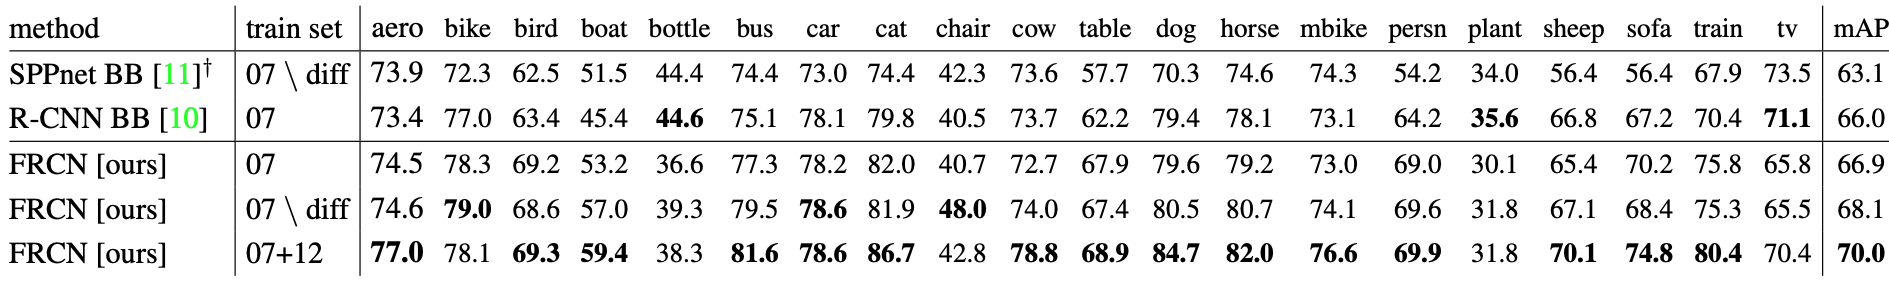
\includegraphics[width=15cm] {images/fast_rcnn_results_1}
        \caption{Kết quả của mô hình Fast R-CNN với các cấu hình khác nhau cùng các mô hình khác trên bộ dữ liệu VOC 2007 test. (Nguồn: \cite{girshick2015fast})}
        \label{fig:fast_rcnn_results_1}
    \end{figure}

    \noindent
    Tiếp theo, mô hình Fast R-CNN cũng có kết quả tốt trên bộ dữ liệu VOC 2010 test.
    Trong hình \ref{fig:fast_rcnn_results_2}, tác giả xét đến hai cấu hình của mô hình Fast R-CNN, các cấu hình này đều có kiến trúc như nhau (đều sử dụng mô hình VGG16 cho thành phần feature extraction module \index{feature extraction module}) nhưng khác nhau về bộ dữ liệu huấn luyện mà mỗi cấu hình sử dụng: \\
    - Cấu hình sử dụng bộ dữ liệu huấn luyện là VOC12 trainval: ký hiệu là \textbf{12} \\
    - Cấu hình sử dụng bộ dữ liệu huấn luyện là sự kết hợp giữa VOC07 trainval, VOC07 test và VOC12 trainval: ký hiệu là \textbf{07 ++ 12} \\
    Trong nhóm các mô hình so sánh, có kết quả của cấu hình tốt nhất của mô hình R-CNN là R-CNN BB.
    Ngoài ra còn có các mô hình BabyLearning (được huấn luyện với bộ dữ liệu độc quyền) và mô hình SegDeepM (được huấn luyện với bộ dữ liệu VOC 12 trainval bổ sung thêm các groundtruth \index{groundtruth} segmentation). \\
    Kết quả của cấu hình \textbf{07 ++ 12} mô hình Fast R-CNN cho mAP cao hơn khoảng 2\% so với các cấu hình và mô hình khác.
    Tuy nhiên, vẫn tồn tại một số lớp đối tượng \index{lớp đối tượng} mà chỉ số AP của cấu hình này làm chưa tốt so với các cấu hình khác hay các mô hình khác như lớp \textit{bottle, plant, sheep, tv ...}.

    \begin{figure}[H]
        \centering
        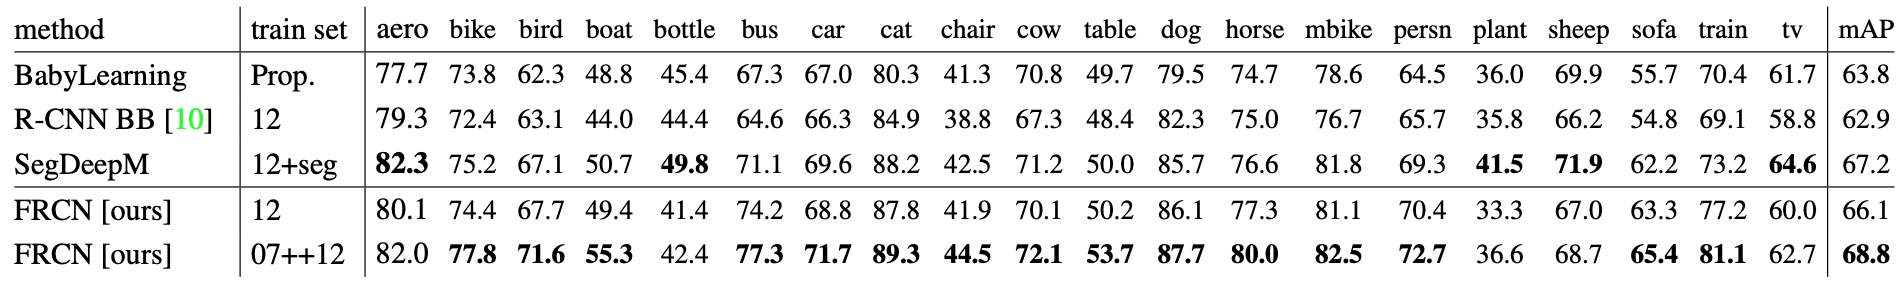
\includegraphics[width=15cm] {images/fast_rcnn_results_2}
        \caption{Kết quả của mô hình Fast R-CNN với các cấu hình khác nhau cùng các mô hình khác trên bộ dữ liệu VOC 2010 test. (Nguồn: \cite{girshick2015fast})}
        \label{fig:fast_rcnn_results_2}
    \end{figure}

    \noindent
    Đối với bộ dữ liệu VOC 2012 test, tác giả vẫn sử dụng hai cấu hình \textbf{12} và \textbf{07 ++ 12} của mô hình Fast R-CNN từ kết quả trên. Nhóm các mô hình so sánh gồm cấu hình R-CNN BB của mô hình R-CNN, mô hình BabyLearning (được huấn luyện với bộ dữ liệu độc quyền) và mô hình NUS\_NIN\_c2000. \\
    Trong hình \ref{fig:fast_rcnn_results_3}, kết quả của cấu hình \textbf{07 ++ 12} mô hình Fast R-CNN cho mAP cao hơn khoảng 3-5\% so với các cấu hình và mô hình khác. \\
    Kết quả này vẫn tồn tại một số lớp đối tượng \index{lớp đối tượng} mà chỉ số AP của cấu hình này làm chưa tốt so với các cấu hình khác hay các mô hình khác như lớp \textit{bottle, plant}.

    \begin{figure}[H]
        \centering
        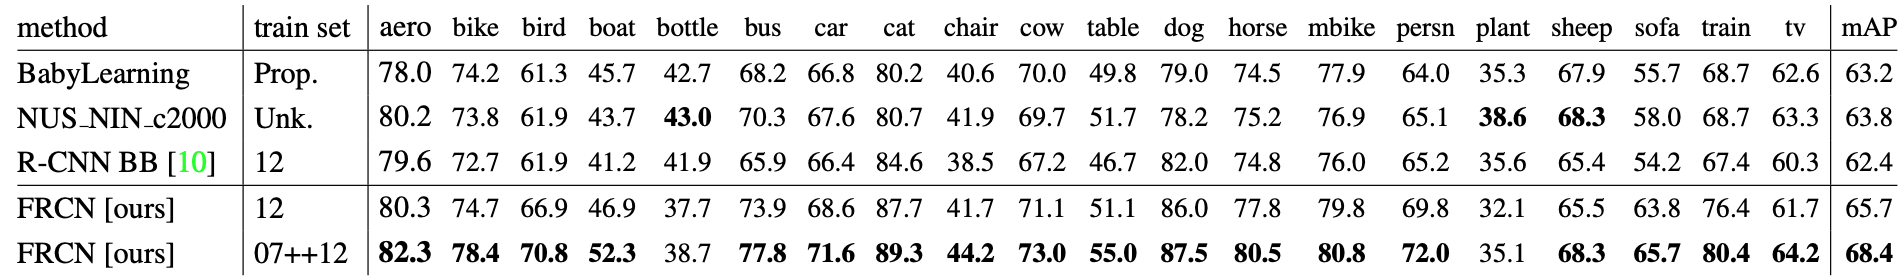
\includegraphics[width=15cm] {images/fast_rcnn_results_3}
        \caption{Kết quả của mô hình Fast R-CNN với các cấu hình khác nhau cùng các mô hình khác trên bộ dữ liệu VOC 2012 test. (Nguồn: \cite{girshick2015fast})}
        \label{fig:fast_rcnn_results_3}
    \end{figure}

    \noindent
    Cuối cùng, tác giả chia sẻ kết quả khi so sánh về mặt tốc độ trong quá trình huấn luyện và quá trình test và đây là một trong số những thành quả chính. \\
    Trong hình \ref{fig:fast_rcnn_results_4}, tác giả so sánh tốc độ xử lý mỗi ảnh trong quá trình huấn luyện và test giữa mô hình Fast R-CNN, R-CNN và SPPnet.
    Cụ thể hơn, trong quá trình huấn luyện, thời gian huấn luyện của mô hình Fast R-CNN giảm tới 8.8 lần so với mô hình R-CNN.
    Trong quá trình test, thời gian mà mô hình Fast R-CNN xử lý một ảnh nhanh hơn tới 146 (khi không sử dụng SVD) và tới 213 lần (khi sử dụng SVD) so với mô hình R-CNN.
    Không những thế, với việc cải thiện đáng kể tốc độ huấn luyện và test, kết quả về độ chính xác của Fast R-CNN vẫn tốt hơn so với R-CNN khi so sánh trên chỉ số mAP.

    \begin{figure}[H]
        \centering
        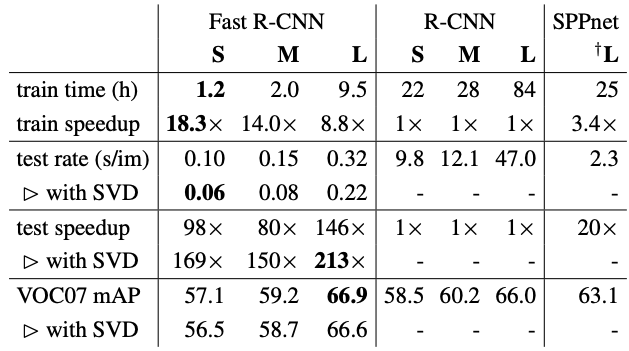
\includegraphics[width=10cm] {images/fast_rcnn_results_4}
        \caption{Kết quả so sánh về mặt tốc độ và độ chính xác giữa các cấu hình khác nhau của mô hình Fast R-CNN, R-CNN và SPPnet. (Nguồn: \cite{girshick2015fast})}
        \label{fig:fast_rcnn_results_4}
    \end{figure}

    \subsubsection*{Vấn đề tồn đọng của mô hình Fast R-CNN}
    Những kết quả vượt bậc về mặt tốc độ của mô hình Fast R-CNN đã giải quyết được vấn đề tồn đọng của R-CNN trong khi vẫn duy trì được độ chính xác cao.
    Tuy nhiên, kiến trúc của mô hình Fast R-CNN vẫn phụ thuộc vào một thuật toán đề xuất khu vực như Selective Search và điều này tạo động lực để các nhà nghiên cứu xây dựng mô hình học sâu thay thế cho các thuật toán này.
}
    \fastrcnn

    \def\fasterrcnn{
    \subsubsection{Mô hình Faster R-CNN}
    Được lấy động lực từ những điểm yếu của mô hình Fast R-CNN, nhóm tác giả đã nghiên cứu và phát triển mô hình Faster R-CNN \cite{ren2015faster} với trung tâm là kiến trúc mô hình Region Proposal Network (gọi tắt là RPN).
    Mô hình Region Proposal Network được kỳ vọng sẽ thay thế hoàn toàn các thuật toán như Selective Search trong thành phần region proposals module \index{region proposals module} của các mô hình two-stage giải quyết bài toán object detection.
    Việc thay thế các thuật toán bằng một kiến trúc học sâu hướng đến việc cải thiện không chỉ tốc độ của mô hình mà còn cải thiện về độ chính xác.

    \noindent
    \textbf{\textit{Kiến trúc mô hình Region Proposal Network}} \\
    Mô hình RPN nhận đầu vào là ảnh với kích thước bất kỳ và trả đầu ra là toạ độ của các khu vực và xác suất khu vực đó là đối tượng nào trong các lớp đối tượng \index{lớp đối tượng}.
    Nhằm tiết kiệm chi phí tính toán, mô hình RPN dùng chung phần feature extraction module \index{feature extraction module} với Fast R-CNN.

    \begin{figure}[H]
        \centering
        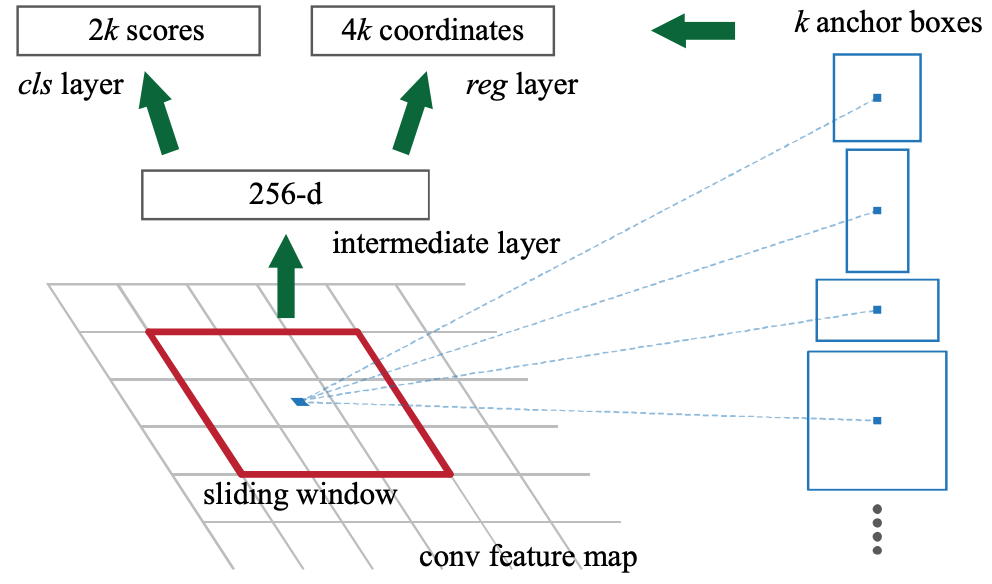
\includegraphics[width=9cm] {images/faster_rcnn_rpn}
        \caption{Kiến trúc mô hình Region Proposal Network (Nguồn: \cite{ren2015faster})}
        \label{fig:faster_rcnn_rpn}
    \end{figure}
    
    \noindent
    Sau khi đưa ảnh qua feature extraction module \index{feature extraction module} và thu được một feature maps, mô hình RPN nhận đầu vào là feature maps \index{feature maps} này và trả đầu ra là các khu vực đề xuất gọi là các anchor \index{anchor}.
    Nhóm tác giả xây dựng phương pháp đề xuất các anchor \index{anchor} dựa trên kích thước và tỷ lệ giữa chiều dài và chiều rộng của anchor \index{anchor}.
    Cụ thể, mô hình RPN đưa feature maps \index{feature maps} qua một lớp Conv \index{lớp Conv} và thu được một feature maps \index{feature maps} mới có kích thước $W x H$.
    Từ đó, nhóm tác giả đề xuất ba kích thước của anchor \index{anchor} và ba tỷ lệ giữa chiều dài và chiều rộng của anchor \index{anchor} tạo ra chín anchor \index{anchor} với mỗi pixels \index{pixels} trên feature maps \index{feature maps} kích thước $W x H$.
    Tổng cộng trên toàn bộ feature maps \index{feature maps} kích thước $W x H$, ta thu được $W x H x 9$ anchor \index{anchor}.
    Các feature maps \index{feature maps} đại diện cho các anchor \index{anchor} này được tiếp tục đưa qua các lớp Conv \index{lớp Conv} để biến đổi về các feature maps \index{feature maps} mới có dạng $(W x H x 9) x 1$ đại diện cho xác suất anchor \index{anchor} đó là object và có dạng $(W x H x 9) x 4$ đại diện cho 4 toạ độ x của góc trái trên, y của góc trái trên, chiều dài và chiều rộng của bounding box \index{bounding box}.

    \noindent
    Một điểm mạnh của RPN so với các mô hình object detection thời bấy giờ đó chính là khả năng dự đoán được các object có kích thước khác nhau và tỷ lệ giữa chiều dài và chiều rộng khác nhau nhờ vào cách cấu hình của anchor \index{anchor}.

    \begin{figure}[H]
        \centering
        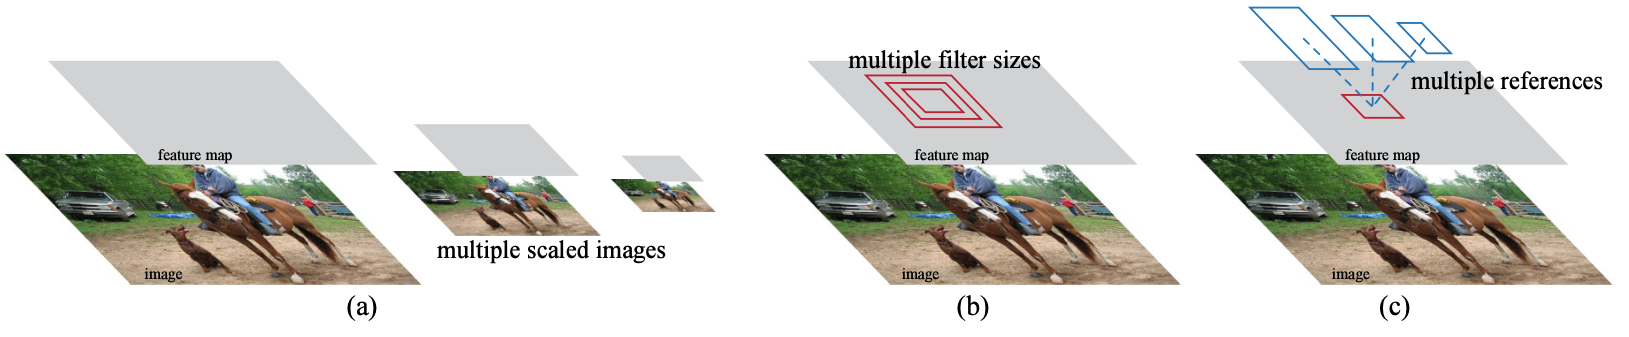
\includegraphics[width=15cm] {images/faster_rcnn_multi_scale_anchor}
        \caption{So sánh các kiến trúc xử lý vấn đề object có kích thước khác nhau và tỷ lệ giữa chiều dài và chiều rộng khác nhau (Nguồn: \cite{ren2015faster})}
        \label{fig:faster_rcnn_multi_scale_anchor}
    \end{figure}

    \noindent
    Một số kiến trúc đã được đề xuất ở thời điểm đó nhưng đều gặp phải rào cản về khối lượng tính toán lớn. \\
    - Kiến trúc đầu tiên là \textit{image/feature pyramids} sử dụng ảnh với nhiều kích thước khác nhau nhằm tạo ra feature maps \index{feature maps} có nhiều kích thước khác nhau.
    Kiến trúc này tốn rất nhiều chi phí tính toán do ta cần xử lý nhiều lần (thường là ba lần) với mỗi ảnh đầu vào khác nhau. \\
    - Kiến trúc thứ hai là \textit{pyramid of filters} đưa cùng một feature maps \index{feature maps} đầu vào qua nhiều khối Conv có kích thước của kernel khác nhau (thường là Conv với kernel 5x7 và Conv với kernel 7x5).
    Kiến trúc này tiết kiệm chi phí tính toán hơn một chút so với kiến trúc đầu tiên và thường được sử dụng kết hợp cùng với kiến trúc đầu tiên. \\
    - Kiến trúc cuối cùng là \textit{pyramid of anchors} được đề xuất trong RPN sử dụng nhiều anchor \index{anchor} với các kích thước khác nhau và tỷ lệ giữa chiều dài và chiều rộng khác nhau.
    Kiến trúc này chỉ tăng một lượng nhỏ chi phí tính toán nếu ta tăng số lượng anchor \index{anchor}, còn phần chi phí tính toán đối với feature maps \index{feature maps} vẫn được giữ nguyên. \\
    Phần cải tiến của RPN đối với object có kích thước khác nhau và tỷ lệ giữa chiều dài và chiều rộng khác nhau chỉ là những cải tiến tại thời điểm đó mà thôi.
    Ở \textit{phần 2.2. Kiến trúc Feature Pyramid Networks}, ta sẽ nghiên cứu một mô hình nâng cấp hơn của Faster R-CNN, giải quyết một cách triệt để hơn vấn đề này.

    \noindent
    \textbf{\textit{Hàm loss và cách train mô hình RPN}} \\
    Để train được mô hình RPN, nhóm tác giả gán cho mỗi anchor \index{anchor} một lớp groundtruth \index{groundtruth} và thiết lập hàm loss đối với từng anchor \index{anchor}.
    Nhóm tác giả gán lớp groundtruth \index{groundtruth} positive cho anchor \index{anchor} dựa theo hai cách sau: \\
    - Những anchor \index{anchor} có chỉ số IoU \index{IoU} lớn nhất đối với một groundtruth \index{groundtruth} bounding box \index{bounding box} được gán là anchor \index{anchor} positive. \\
    - Những anchor \index{anchor} có chỉ số IoU \index{IoU} lớn hơn 0.7 đối với một groundtruth \index{groundtruth} bounding box \index{bounding box} được gán là anchor \index{anchor} positive. \\
    Với hai cách như trên, một groundtruth \index{groundtruth} bounding box \index{bounding box} có thể gán được cho nhiều anchor \index{anchor} khác nhau.
    Ngoài ra, nhóm tác giả cũng gán lớp groundtruth \index{groundtruth} negative cho các anchor \index{anchor} không phải là positive và có chỉ số IoU \index{IoU} nhỏ hơn 0.3 đối với một groundtruth \index{groundtruth} bounding box \index{bounding box}. \\
    Từ đó, mô hình Faster R-CNN tối ưu hàm loss sau:

    \begin{equation}
        \label{eq:faster_rcnn_loss}
        L(\{p_i\}, \{t_i\}) = \frac{1}{N_{cls}}\sum_i L_{cls}(p_i, p^{*}_i) + \lambda\frac{1}{N_{reg}}\sum_i  p^{*}_i L_{reg}(t_i, t^{*}_i).
    \end{equation}

    \noindent
    trong đó: \\
    - \textit{i} là chỉ số của từng anchor \index{anchor}. \\
    - \textit{$p_i$} là xác suất mà anchor \index{anchor} chứa đối tượng. \\
    - \textit{$p^{*}_i$} là groundtruth \index{groundtruth} của anchor \index{anchor} (là 1 nếu anchor \index{anchor} đó được gán là chứa đối tượng, là 0 nếu anchor \index{anchor} đó được gán là không chứa đối tượng). \\
    - \textit{$t_i$} là vector gồm 4 giá trị đại diện cho toạ độ của khu vực mà mô hình RPN đề xuất. \\
    - \textit{$t^{*}_i$} là vector gồm 4 giá trị đại diện cho toạ độ của groundtruth \index{groundtruth} bounding box \index{bounding box} tương ứng với anchor \index{anchor} đó. \\
    Hàm loss trên gồm các thành phần: \\
    - \textit{$L_{cls}$}: là hàm loss phân lớp thông thường giúp xác định anchor \index{anchor} có chứa đối tượng hay không. \\
    - \textit{$L_{reg}$}: là hàm loss hồi quy đối với các anchor \index{anchor} positive, giúp tinh chỉnh toạ độ của khu vực mà mô hình đề xuất.
    Cụ thể, nhóm tác giả sử dụng $L_{reg}(t_i, t^{*}_i)=L_1(t_i - t^{*}_i)$ giống với hàm loss sử dụng trong mô hình Fast R-CNN \cite{girshick2015fast}.

    \noindent
    Mô hình RPN được thiết kế để có thể train cùng với quá trình train object detection từ đó giúp kết quả đề xuất khu vực trở nên chính xác hơn.
    Tuy nhiên, có một vấn đề nảy sinh khi sử dụng mô hình RPN cho việc đề xuất khu vực, đó là mô hình sẽ đề xuất ra nhiều các anchor \index{anchor} negative hơn rất nhiều so với số anchor \index{anchor} positive.
    Việc train mô hình trên từng anchor \index{anchor} kết hợp với hiện tượng trên sẽ khiến cho tổng quan mô hình object detection bị mất cân bằng dữ liệu \index{mất cân bằng dữ liệu}.
    Ngoài ra, việc train mô hình với toàn bộ số anchor \index{anchor} được đề xuất ra cũng sẽ khiến cho khối lượng tính toán lớn và thời gian kéo dài quá trình train mô hình.
    Từ đó, nhóm tác giả đề xuất việc lựa chọn ngẫu nhiên 256 anchor \index{anchor} trên mỗi ảnh để thực hiện việc tính loss. Việc lựa chọn này giúp tỷ lệ anchor \index{anchor} positive và negative trở nên cân bằng hơn và giảm thiểu bởi những phần khối lượng tính toán dư thừa.

    \noindent
    \textbf{\textit{Sự kết hợp giữa mô hình Region Proposal Network và Fast R-CNN}} \\
    Nhóm tác giả cho rằng, việc train mô hình RPN và Fast R-CNN cần phải diễn ra đồng thời, vì từ đó, việc chia sẻ chung thành phần backbone Conv mới trở nên hiệu quả.

    \begin{figure}[H]
        \centering
        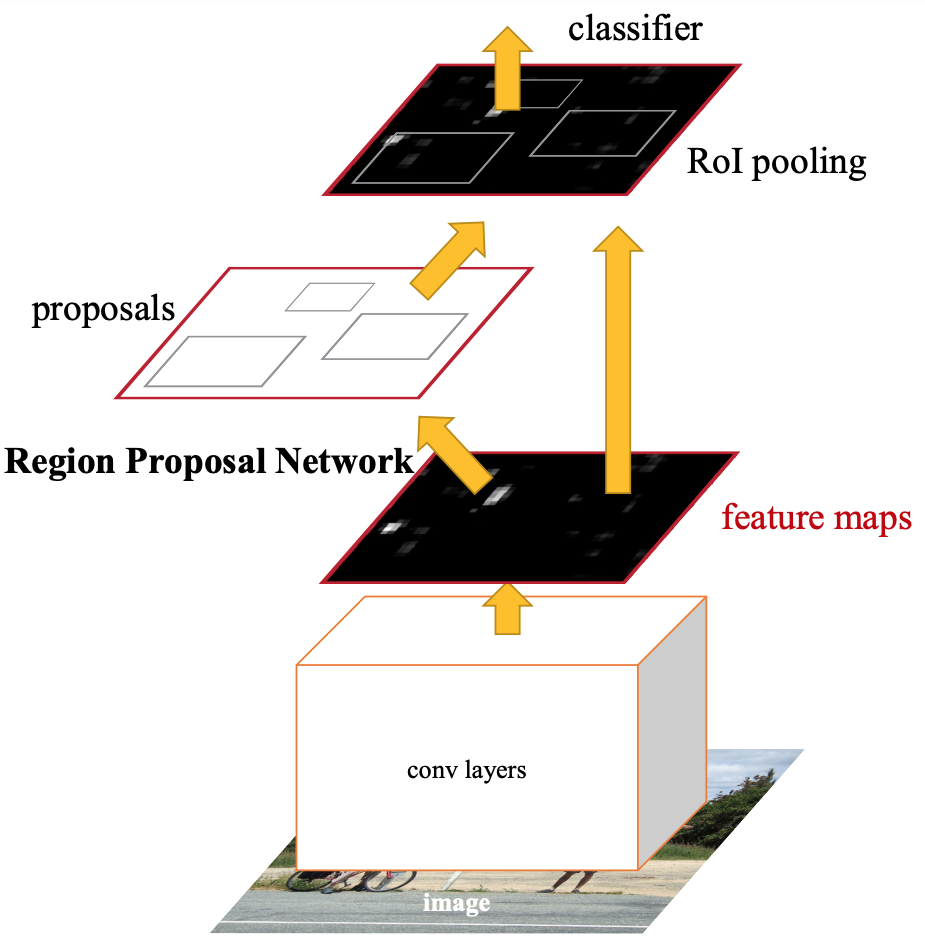
\includegraphics[width=10cm] {images/faster_rcnn_model}
        \caption{Toàn cảnh sự kết hợp của mô hình Region Proposal Network và Fast R-CNN tạo ra mô hình Faster R-CNN (Nguồn: \cite{ren2015faster})}
        \label{fig:faster_model}
    \end{figure}

    \noindent
    Nhóm tác giả nêu ra ba phương án để train mô hình RPN kết hợp với Fast R-CNN: \\
    - Cách 1: \textit{Alternating training}: Nhóm tác giả train mô hình RPN trước sử dụng những hàm loss của RPN nói trên.
    Sau khi train xong mô hình RPN, tác giả sử dụng những khu vực được đề xuất bởi RPN để train mô hình Fast R-CNN.
    Mô hình backbone sau khi được train bởi Fast R-CNN tiếp tục được sử dụng để train mô hình RPN mới và vòng lặp này tiếp tục diễn ra cho đến khi kết quả của mô hình hội tụ. \\
    - Cách 2: \textit{Approximate joint training}: Phương pháp này kết hợp RPN và Fast R-CNN thành một mô hình duy nhất trong quá trình train.
    Các khu vực được đề xuất bởi RPN được coi như là tất định đối với nhánh Fast R-CNN và khiến cho phương pháp train này được gọi là \textit{approximate} bởi vì những thông tin từ nhánh Fast R-CNN sẽ không được cập nhật cho nhánh RPN.
    Quá trình backprop được thực hiện độc lập giữa RPN và Fast R-CNN, riêng phần backbone chung của RPN và Fast R-CNN được cập nhật theo giá trị hàm loss của cả RPN và Fast R-CNN.
    Phương pháp này đạt hiệu quả thấp hơn chút so với \textit{Alternating training} tuy nhiên thời gian train được giảm 25 - 50\%. \\
    - Cách 3: \textit{Non-approximate joint training}: Phương pháp này cải thiện được vấn đề \textit{approximate} tồn đọng của \textit{Approximate joint training}.
    Tuy nhiên, để làm được điều này, nhóm tác giả cần tinh chỉnh lại lớp RoI pooling trong Fast R-CNN để có thể update cho cả các thành phần của mô hình Fast R-CNN và RPN.
    Điều này nằm ngoài nội dung của nghiên cứu này nên nhóm tác giả không đề cập kỹ hơn.

    \noindent
    Tóm lại, nhóm tác giả dựa vào phương pháp \textit{Alternating training} và thực hiện quá trình train gồm 4 bước như sau: \\
    - Bước 1: Nhóm tác giả khởi tạo mô hình RPN với pretrained ImageNet và train mô hình RPN. \\
    - Bước 2: Nhóm tác giả khởi tạo mô hình Fast R-CNN với pretrained ImageNet và train mô hình Fast R-CNN với các khu vực được đề xuất bởi RPN. \\
    - Bước 3: Nhóm tác giả khởi tạo lại mô hình RPN nhưng sử dụng phần backbone đã được train từ bước 2.
    Nhóm tác giả chỉ train những lớp riêng của mô hình RPN và không cập nhật cho phần backbone. \\
    - Bước 4: Nhóm tác giả finetune lại những lớp riêng của mô hình Fast R-CNN với các khu vực được đề xuất bởi RPN và thu được mô hình Faster R-CNN cuối cùng. \\
    Nhóm tác giả cũng đã lặp lại 4 bước trên vài lần nhưng kết quả không thay đổi quá nhiều.

    \noindent
    \textbf{\textit{Kết quả của mô hình Faster R-CNN}} \\
    Đầu tiên, trong hình \ref{fig:faster_rcnn_results_1}, kết quả của mô hình Fast R-CNN sử dụng RPN, backbone ZF-Net và dùng chung backbone giữa nhánh RPN và nhánh Fast R-CNN (\textbf{RPN+ZF, shared}) tốt hơn trên chỉ số mAP so sánh với việc sử dụng thuật toán Selective Search \textbf{SS} và EdgeBoxes \textbf{EB} trên bộ dữ liệu VOC 2007 test. Trong đó, số lượng khu vực được đề xuất trong quá trình train được thống kê tại cột \textbf{\# boxes}, trong quá trình test được thống kê tại cột \textbf{\# proposals}.

    \begin{figure}[H]
        \centering
        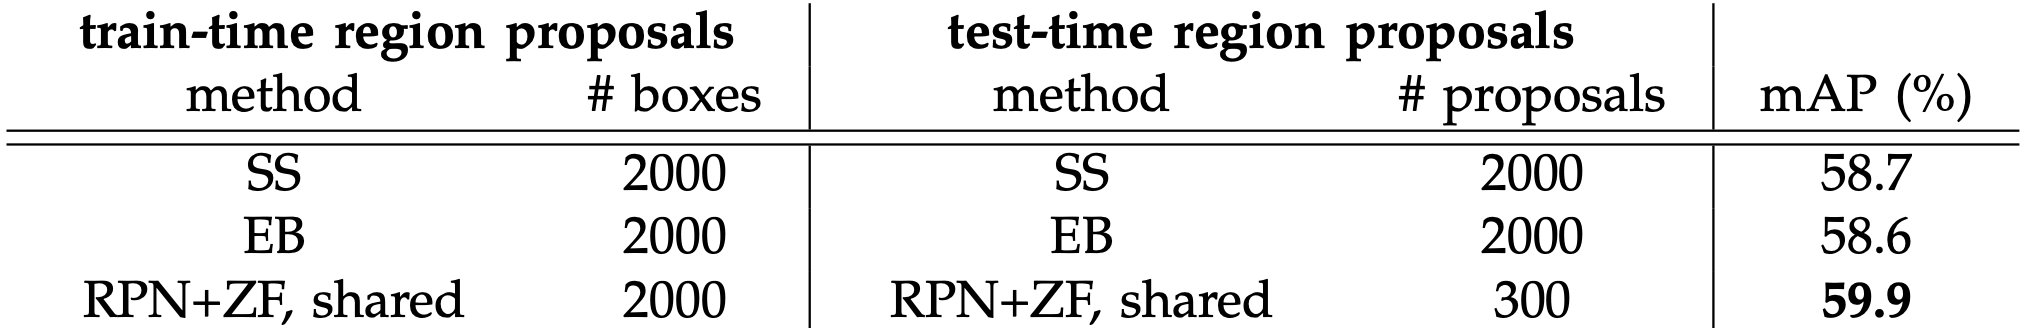
\includegraphics[width=10cm] {images/faster_rcnn_results_1}
        \caption{Kết quả của mô hình Fast R-CNN sử dụng RPN so sánh với việc sử dụng thuật toán Selective Search và EdgeBoxes trên bộ dữ liệu VOC 2007 test. (Nguồn: \cite{ren2015faster})}
        \label{fig:faster_rcnn_results_1}
    \end{figure}

    \noindent
    Tiếp theo, trong hình \ref{fig:faster_rcnn_results_2}, nhóm tác giả so sánh kết quả của các mô hình Faster R-CNN (dùng backbone là VGG-16, ký hiệu là \textbf{RPN + VGG}) với mô hình Fast R-CNN sử dụng thuật toán Selective Search trên bộ dữ liệu VOC 2007 test nhưng với các bộ dữ liệu train khác nhau. \\
    - Cấu hình sử dụng riêng hai backbone khác nhau giữa nhánh RPN và nhánh Fast R-CNN: ký hiệu là \textbf{unshared} \\
    - Cấu hình sử dụng chung backbone giữa nhánh RPN và nhánh Fast R-CNN: ký hiệu là \textbf{shared} \\
    - Cấu hình sử dụng bộ dữ liệu train là VOC07 trainval: ký hiệu là \textbf{07} \\
    - Cấu hình sử dụng bộ dữ liệu train là sự kết hợp giữa VOC07 trainval và VOC12 trainval: ký hiệu là \textbf{07+12} \\
    - Cấu hình sử dụng bộ dữ liệu train là sự kết hợp giữa VOC07 trainval, VOC12 trainval và bộ dữ liệu MS-COCO: ký hiệu là \textbf{COCO+07+12} \\
    Trong đó, số lượng khu vực được đề xuất trong quá trình test được thống kê tại cột \textbf{\# proposals}. \\
    Kết quả mô hình \textbf{RPN + VGG, unshared, 07} đạt chỉ số mAP là 68.5\%, tốt hơn so với 66.9\% của mô hình \textbf{SS, 07}.
    Kết quả mô hình \textbf{RPN + VGG, shared, 07+12} đạt chỉ số mAP là 73.2\%, tốt hơn so với 70.0\% của mô hình \textbf{SS, 07+12}.
    Và mô hình \textbf{RPN + VGG, shared, COCO+07+12} đạt chỉ số mAP cao nhất là 78.8\%, điều này khá dễ hiểu khi mô hình sử dụng nhiều dữ liệu train hơn sẽ cho kết quả tốt hơn.

    \begin{figure}[H]
        \centering
        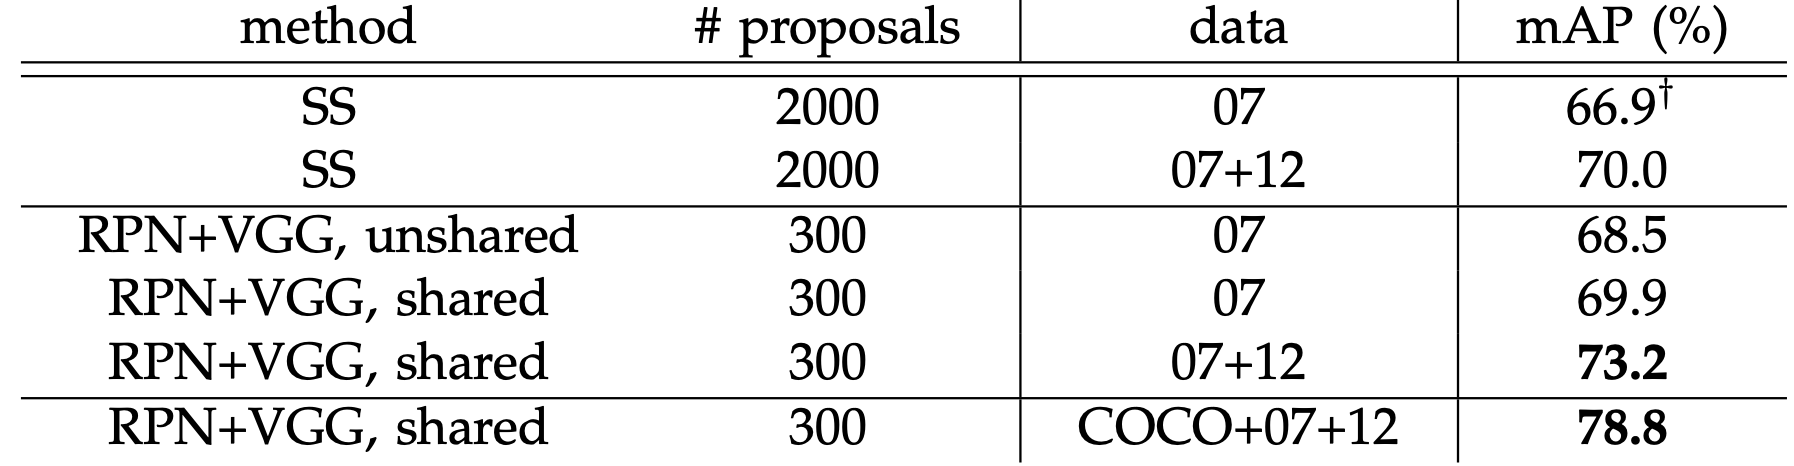
\includegraphics[width=10cm] {images/faster_rcnn_results_2}
        \caption{Kết quả của mô hình Fast R-CNN sử dụng RPN và backbone VGG-16 so sánh với mô hình Fast R-CNN sử dụng thuật toán Selective Search trên bộ dữ liệu VOC 2007 test với các bộ dữ liệu train khác nhau. (Nguồn: \cite{ren2015faster})}
        \label{fig:faster_rcnn_results_2}
    \end{figure}

    \noindent
    Tiếp theo, trong hình \ref{fig:faster_rcnn_results_3}, nhóm tác giả so sánh kết quả của các mô hình Faster R-CNN (dùng backbone là VGG-16, ký hiệu là \textbf{RPN + VGG}) với mô hình Fast R-CNN sử dụng thuật toán Selective Search trên bộ dữ liệu VOC 2012 test nhưng với các bộ dữ liệu train khác nhau. \\
    - Cấu hình sử dụng chung backbone giữa nhánh RPN và nhánh Fast R-CNN: ký hiệu là \textbf{shared} \\
    - Cấu hình sử dụng bộ dữ liệu train là VOC12 trainval: ký hiệu là \textbf{12} \\
    - Cấu hình sử dụng bộ dữ liệu train là sự kết hợp giữa VOC07 trainval+test và VOC12 trainval: ký hiệu là \textbf{07++12} \\
    - Cấu hình sử dụng bộ dữ liệu train là sự kết hợp giữa VOC07 trainval+test, VOC12 trainval và bộ dữ liệu MS-COCO: ký hiệu là \textbf{COCO+07+12} \\
    Trong đó, số lượng khu vực được đề xuất trong quá trình test được thống kê tại cột \textbf{\# proposals}. \\
    Kết quả mô hình \textbf{RPN + VGG, shared, 12} đạt chỉ số mAP là 67.0\%, tốt hơn so với 65.7\% của mô hình \textbf{SS, 12}.
    Kết quả mô hình \textbf{RPN + VGG, shared, 07++12} đạt chỉ số mAP là 70.4\%, tốt hơn so với 68.4\% của mô hình \textbf{SS, 07++12}.
    Và mô hình \textbf{RPN + VGG, shared, COCO+07++12} đạt chỉ số mAP cao nhất là 75.9\%, điều này khá dễ hiểu khi mô hình sử dụng nhiều dữ liệu train hơn sẽ cho kết quả tốt hơn.

    \begin{figure}[H]
        \centering
        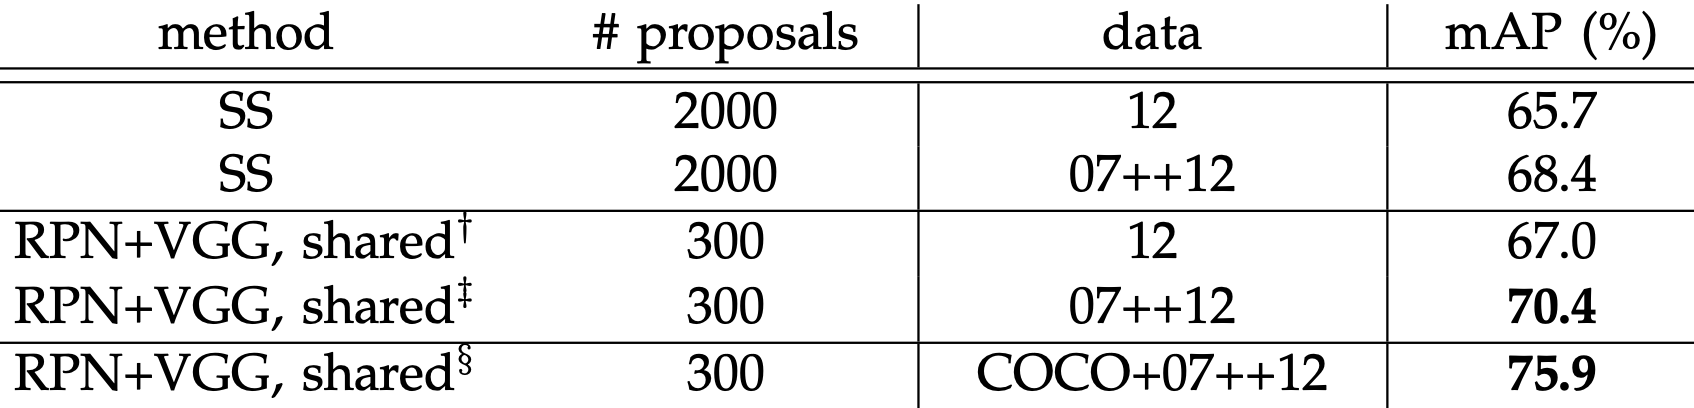
\includegraphics[width=10cm] {images/faster_rcnn_results_3}
        \caption{Kết quả của mô hình Fast R-CNN sử dụng RPN và backbone VGG-16 so sánh với mô hình Fast R-CNN sử dụng thuật toán Selective Search trên bộ dữ liệu VOC 2012 test với các bộ dữ liệu train khác nhau. (Nguồn: \cite{ren2015faster})}
        \label{fig:faster_rcnn_results_3}
    \end{figure}

    \noindent
    Cuối cùng, so sánh về mặt tốc độ, nhóm tác giả so sánh kết quả của các mô hình Faster R-CNN (dùng backbone là VGG-16, ký hiệu là \textbf{VGG, RPN + Fast R-CNN}), mô hình Faster R-CNN (dùng backbone là ZF-Net, ký hiệu là \textbf{ZF, RPN + Fast R-CNN}) với mô hình Fast R-CNN sử dụng thuật toán Selective Search (dùng backbone là VGG-16, ký hiệu là \textbf{VGG, SS + Fast R-CNN}).
    Trong đó, thời gian (tính theo đơn vị ms) xử lý lớp conv được thống kê tại cột \textbf{conv}, thời gian đề xuất các khu vực được thống kê tại cột \textbf{proposals}, thời gian xử lý các bước như NMS, lớp pooling, lớp fully connected \index{lớp fully connected} và lớp softmax được thống kê tại cột \textbf{region-wise}, tổng thời gian xử lý toàn bộ được thống kê tại cột \textbf{total}, số lượng ảnh xử lý trong một giây được thống kê tại cột \textbf{rate}. \\
    Kết quả, mô hình \textbf{VGG, RPN + Fast R-CNN} nhanh hơn \textbf{VGG, SS + Fast R-CNN} gần 10 lần, trong đó, thời gian đề xuất khu vực được tiết kiệm tới 150 lần.
    Mô hình \textbf{ZF, RPN + Fast R-CNN} thậm chí còn nhanh gấp gần bốn lần mô hình \textbf{VGG, RPN + Fast R-CNN}, đạt số khung hình trên một giây là 17 fps.

    \begin{figure}[H]
        \centering
        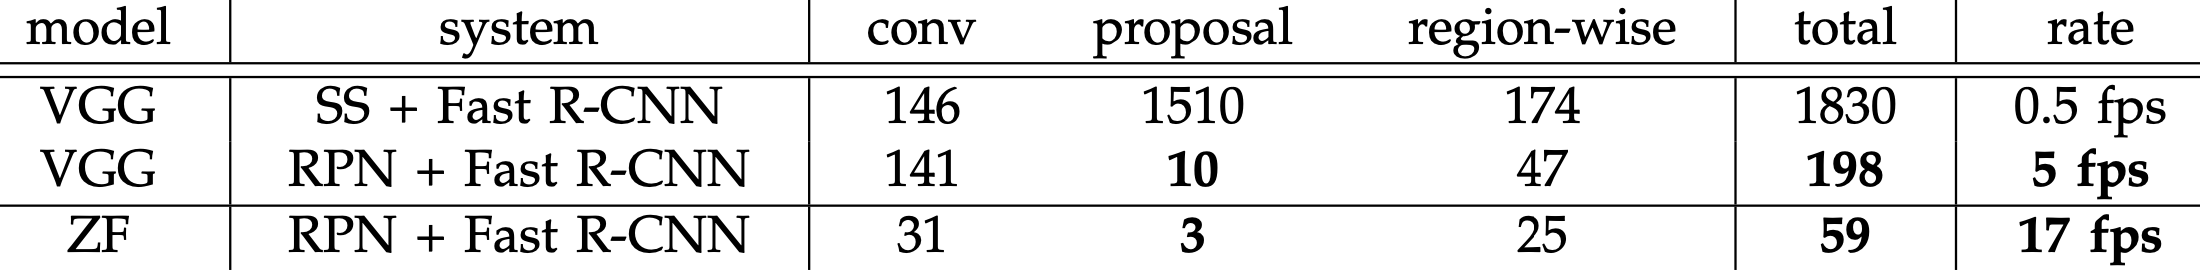
\includegraphics[width=10cm] {images/faster_rcnn_results_4}
        \caption{Toàn cảnh sự kết hợp của mô hình Region Proposal Network và Fast R-CNN tạo ra mô hình Faster R-CNN (Nguồn: \cite{ren2015faster})}
        \label{fig:faster_rcnn_results_4}
    \end{figure}

    \noindent
    \textbf{\textit{Vấn đề tồn đọng của mô hình Faster R-CNN}} \\
    Kết quả của mô hình Faster R-CNN và tâm điểm là kiến trúc RPN giúp thay thế thuật toán Selective Search đã giúp cho Faster R-CNN đạt độ chính xác cao hơn so với mô hình Fast R-CNN sử dụng Selective Search.
    Hơn nữa, RPN giúp cho Faster R-CNN nhanh hơn tới 10 lần so với cấu hình tương tự Fast R-CNN sử dụng Selective Search.
    Điều này giúp cho Faster R-CNN cho đến nay vẫn là một mô hình tốt để giải quyết bài toán object detection, vừa đạt độ chính xác cao, vừa có tốc độ tương đối tốt.
    Tuy nhiên, cho đến thời điểm thực hiện luận văn này, đã có nhiều mô hình khác hiện đại hơn chỉ ra những vấn đề tồn đọng của Faster R-CNN như độ chính xác cần phải cải thiện thêm hay tốc độ chưa đạt đến ngưỡng chạy trong thời gian thực. 
}
    \fasterrcnn

    \subsection{Kiến trúc Feature Pyramid Network}

    \subsection{Các mô hình single-stage giải quyết bài toán object detection}
    \subsection{Mô hình SSD}

    \subsection{Nhóm các mô hình YOLO}

    \subsection{Mô hình RetinaNet}
    \subsubsection{Kiến trúc Feature Pyramid Network}
    - Nhắc thêm đến backbone ResNet
    \subsubsection{Hàm Focal loss}
}